\documentclass[a4paper,11pt]{article} 
\usepackage[francais]{babel}
\usepackage[T1]{fontenc} 
\usepackage[utf8]{inputenc} 
\usepackage{graphicx}
\usepackage{color}
\usepackage{hyperref}
\usepackage{bookmark}
\usepackage{array}
\usepackage{geometry}
\geometry{a4paper, margin=1in}

\begin{document}

\begin{figure}

\includegraphics[width=0.3\textwidth]{images/logolemansU.png}
\hspace{150pt} 
\includegraphics[width=0.3\textwidth]{images/logo_ic2.png} 
\end{figure}

\title{\textbf{\color{blue} Le Mans Université}\color{black}
\\ Licence Informatique \textit{3ème année}
\\ Module IHM
\\ \textit{meilleursitepourreserverdesvacancesaveclevoletl'hotelet\\lesactivitesetquiprendleschiensetquiprendlesenfantspascher}
\\ \textbf{Personas}}
\author{LEPINE François\\BORRY Lenny\\GHRIB Yacine\\VEAU-BIGOT Damien}
\date{\today} 
\maketitle 
\newpage

\tableofcontents
\newpage


\section{Introduction}
Un persona est une représentation fictive et détaillée d'un utilisateur ou client type, basée sur des données réelles, des recherches et des hypothèses éclairées.
\subsection{Description détaillée}
\noindent Description type:
\begin{itemize}
    \item \textbf{Nom:} Un nom fictif pour le rendre plus humain.
    \item \textbf{Données démographiques:} Âge, sexe, localisation, statut familial, etc.
    \item \textbf{Occupation et situation professionnelle:}  Rôle, niveau d'expérience, secteur d'activité.
    \item \textbf{Besoins et objectifs:} Ce que l'utilisateur souhaite accomplir.
    \item \textbf{Frustrations et points de douleur:} Ce qui complique leur vie ou leur expérience.
    \item \textbf{Comportements et préférences:} Comment ils interagissent avec des produits, services ou technologies.
\end{itemize}

\section{Personas}

\subsection{Persona - TYPE 1}
\begin{minipage}{0.6\textwidth} % 60% de la largeur pour le texte
    \textbf{Nom:} Dimitri Mpondo-Guibert.\\
    \textbf{Âge:} 28 ans.\\
    \textbf{Situation:} En couple.\\
    \textbf{Profession:} Huissier de justice.\\
    \textbf{Statut familial:} Marié depuis 2 ans, a récemment adopté un chien.\\
    \textbf{Besoins et objectifs:} Il souhaite pouvoir voyager, Il veut pouvoir avoir accès aux vols, aux logements, aux localisations et aux activités sur le même site.\\
    \textbf{Frustrations et points de douleur:} C'est une personne assez paresseuse, il n'a pas envie de chercher par lui-même.\\
\end{minipage}%
\hspace{1cm}
\begin{minipage}{0.3\textwidth} % 30% de la largeur pour l'image
    \begin{center}
        
\includegraphics[width=\textwidth]{images/Dimitri.jpeg} % Remplacer 'image.jpeg' par le chemin de votre image
    \end{center}
\end{minipage}

\subsection{Persona - TYPE 2}
\begin{minipage}{0.6\textwidth} % 60% de la largeur pour le texte
    \textbf{Nom:} Léa Fontaine.\\
    \textbf{Âge:} 32 ans.\\
    \textbf{Situation:} Célibataire.\\
    \textbf{Profession:} Graphiste freelance.\\
    \textbf{Statut familial:} Vit seule dans un appartement en centre-ville, possède un chat.\\
    \textbf{Besoins et objectifs:} Cherche une plateforme intuitive pour planifier des séjours culturels, trouver des musées, expositions, et hébergements artistiques.\\
    \textbf{Frustrations et points de douleur:} Déteste les sites web complexes avec trop d'options, manque souvent de temps pour planifier ses voyages.\\
\end{minipage}%
\hspace{1cm}
\begin{minipage}{0.3\textwidth} % 30% de la largeur pour l'image
    \begin{center}
        
\includegraphics[width=\textwidth]{images/femmeabarbe.jpg} % Remplacer 'image.jpeg' par le chemin de votre image
    \end{center}
\end{minipage}



\subsection{Persona - TYPE 3}
\begin{minipage}{0.6\textwidth} % 60% de la largeur pour le texte
\textbf{Nom:} Ahmed Belkacem.\\
\textbf{Âge:} 45 ans.\\
\textbf{Situation:} Divorcé.\\
\textbf{Profession:} Entrepreneur dans le domaine de la restauration.\\
\textbf{Statut familial:} Père de deux adolescents qu'il garde une semaine sur deux.\\
\textbf{Besoins et objectifs:} Veut organiser des vacances en famille avec des activités adaptées pour les adolescents et des moments de détente pour lui.\\
\textbf{Frustrations et points de douleur:} Trouve souvent les offres pour familles peu adaptées aux adolescents et trop coûteuses.\\
\end{minipage}%
\hspace{1cm}
\begin{minipage}{0.3\textwidth} % 30% de la largeur pour l'image
    \begin{center}
        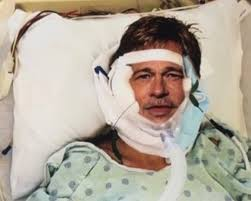
\includegraphics[width=\textwidth]{images/Cbradpitt.jpeg} % Remplacer 'image.jpeg' par le chemin de votre image
    \end{center}
\end{minipage}



\subsection{Persona - TYPE 4}
\begin{minipage}{0.6\textwidth} % 60% de la largeur pour le texte
\textbf{Nom:} Sophie Delacroix.\\
\textbf{Âge:} 23 ans.\\
\textbf{Situation:} Étudiante en master.\\
\textbf{Profession:} Travaille à temps partiel comme serveuse.\\
\textbf{Statut familial:} Vit en colocation avec trois amis.\\
\textbf{Besoins et objectifs:} Recherche des escapades abordables pour explorer de nouvelles villes tout en respectant son budget étudiant.\\
\textbf{Frustrations et points de douleur:} Difficulté à trouver des offres économiques combinant transports et logements.\\
\end{minipage}%
\hspace{1cm}
\begin{minipage}{0.3\textwidth} % 30% de la largeur pour l'image
    \begin{center}
        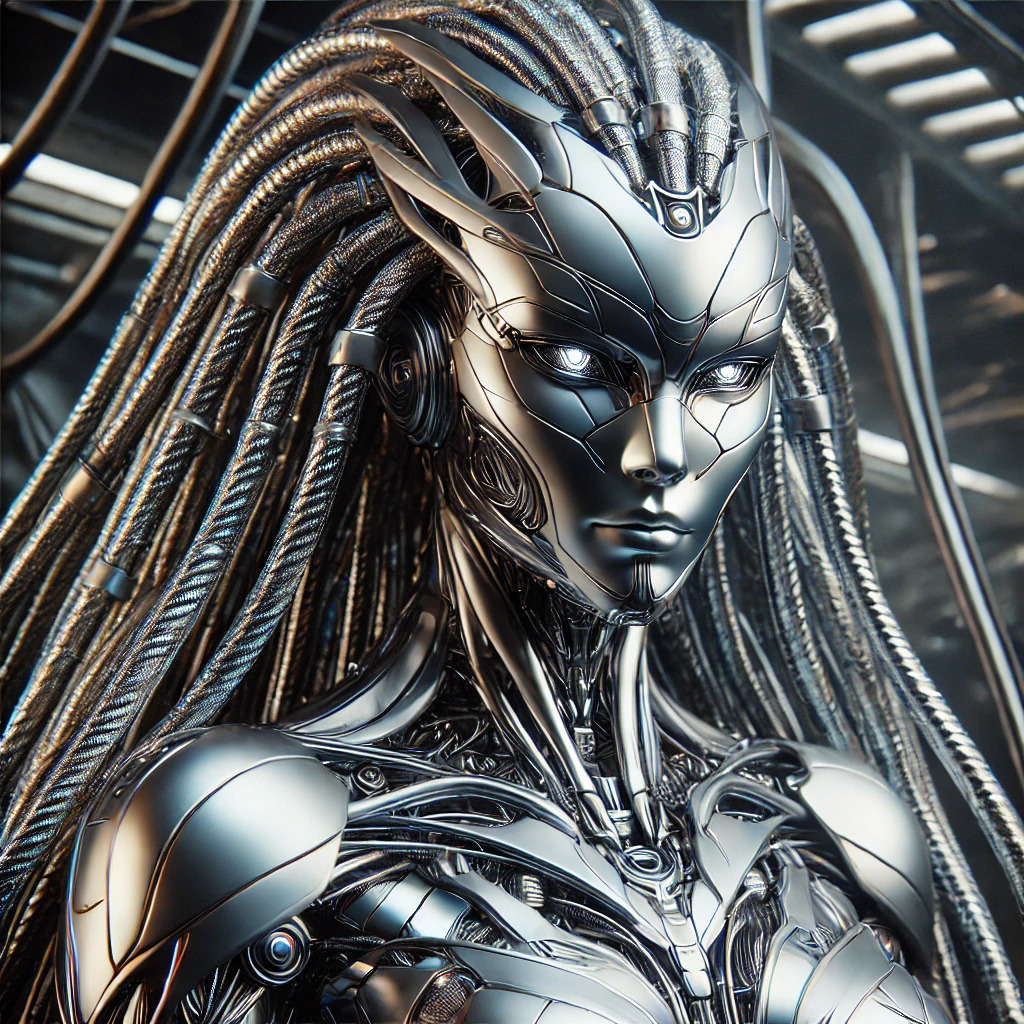
\includegraphics[width=\textwidth]{images/autobott.jpeg} % Remplacer 'image.jpeg' par le chemin de votre image
    \end{center}
\end{minipage}



\subsection{Persona - TYPE 5}
\begin{minipage}{0.6\textwidth} % 60% de la largeur pour le texte
\textbf{Nom:} Marc Dupuis.\\
\textbf{Âge:} 54 ans.\\
\textbf{Situation:} Marié.\\
\textbf{Profession:} Responsable des ventes dans une grande entreprise.\\
\textbf{Statut familial:} Père d'un enfant étudiant à l'étranger.\\
\textbf{Besoins et objectifs:} Souhaite organiser des voyages professionnels et personnels tout en optimisant le temps et la logistique.\\
\textbf{Frustrations et points de douleur:} Perd du temps avec les outils de réservation fragmentés qui ne synchronisent pas bien son agenda.\\
\end{minipage}%
\hspace{1cm}
\begin{minipage}{0.3\textwidth} % 30% de la largeur pour l'image
    \begin{center}
        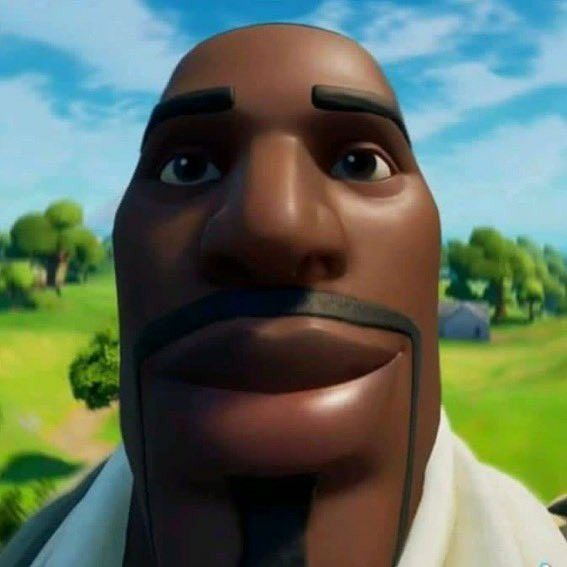
\includegraphics[width=\textwidth]{images/pnj.jpg} % Remplacer 'image.jpeg' par le chemin de votre image
    \end{center}
\end{minipage}


\end{document}
